\documentclass[10pt]{article}
\usepackage[margin=0.7in, top=0.6in, bottom=0.65in]{geometry}
\usepackage{titlesec}
\usepackage{enumitem}
\usepackage{hyperref}
\usepackage{xcolor}
\usepackage{amsmath}
\usepackage{parskip}
\usepackage{graphicx}
\usepackage{tabularx}
\usepackage{booktabs}
\usepackage{tikz}
\usetikzlibrary{shapes.geometric, arrows.meta, positioning, fit}

\titleformat{\section}{\normalfont\bfseries\normalsize}{}{0em}{}
\titlespacing*{\section}{0pt}{6pt}{2pt}
\titleformat{\subsection}{\normalfont\bfseries\small}{}{0em}{}
\titlespacing*{\subsection}{0pt}{4pt}{1pt}
\setlength{\parskip}{3pt}
\setlength{\parindent}{0pt}

\hypersetup{colorlinks=true, linkcolor=blue!70!black, urlcolor=blue!70!black}

\usepackage{fancyhdr}
\pagestyle{fancy}\fancyhf{}
\renewcommand{\headrulewidth}{0pt}
\fancyfoot[C]{\thepage}
\fancyhead[L]{\small\textit{EGN 6217 -- Applied Deep Learning}}
\fancyhead[R]{\small\textit{Deliverable 1.2 -- Technical Blueprint}}

\begin{document}

\begin{center}
    {\Large \textbf{FinReason --- Technical Blueprint}} \\[4pt]
    {\normalsize Deliverable 1.2: From Pitch to Prototype} \\[3pt]
    {\small Om --- MS in AI Systems, University of Florida --- Spring 2026}
\end{center}
\vspace{2pt}\hrule\vspace{6pt}

\section{a. Problem Context and Project Summary}

Financial analysts spend hours extracting and computing figures from earnings reports---year-over-year revenue growth, operating margin changes, percentage-of-total breakdowns. Large language models promise to automate this, but they consistently fail at the math: they hallucinate numbers, confuse table rows, and skip arithmetic steps. FinReason addresses this by applying reinforcement learning with verifiable rewards (GRPO) to a small LLM, training it to produce correct numerical answers over real S\&P 500 financial filings. The reward is simple and deterministic: right number $= +1$, wrong $= 0$. No learned reward model, no human annotation---just ground-truth answer verification.

\section{b. Dataset}

\renewcommand{\arraystretch}{1.15}
\begin{tabularx}{\textwidth}{@{}p{2cm}X@{}}
\toprule
\textbf{Property} & \textbf{Details} \\
\midrule
Source & \textbf{FinQA} (Chen et al., EMNLP 2021). HuggingFace: \texttt{ibm-research/finqa} \\
Type & Tabular + textual financial data with numerical QA pairs \\
Size & 8,281 QA pairs over 2,789 S\&P 500 earnings reports \\
Format & JSON with fields: \texttt{pre\_text}, \texttt{table} (2D array), \texttt{post\_text}, \texttt{qa} (nested dict with \texttt{question}, \texttt{exe\_ans}, \texttt{program}) \\
Access & Public, Creative Commons 4.0. No institutional agreement. Downloads via \texttt{datasets} library in seconds. \\
Split & Train: ${\sim}$6,200 / Validation: ${\sim}$880 / Test: ${\sim}$1,150 \\
Secondary & \textbf{TAT-QA} (Zhu et al., ACL 2021): 16,552 questions for out-of-distribution evaluation \\
\midrule
\multicolumn{2}{@{}l}{\textbf{Preprocessing Challenges}} \\
\midrule
\multicolumn{2}{@{}p{\textwidth}}{Tables must be flattened from 2D arrays into pipe-delimited text strings. Contexts vary from 200 to 4,000+ characters and must be truncated to fit 1,024 tokens. Answers appear in diverse formats (\$1.45B, 1,452 million, (3.5) for negatives) requiring a robust normalization pipeline.} \\
\midrule
\multicolumn{2}{@{}l}{\textbf{Ethical / Privacy Considerations}} \\
\midrule
\multicolumn{2}{@{}p{\textwidth}}{All data is derived from publicly filed SEC documents. No PII, no proprietary data, no scraping. The dataset was created by financial experts at UPenn and published through peer review.} \\
\bottomrule
\end{tabularx}

\section{c. Planned Architecture}

\subsection{Pipeline Diagram}

\begin{center}
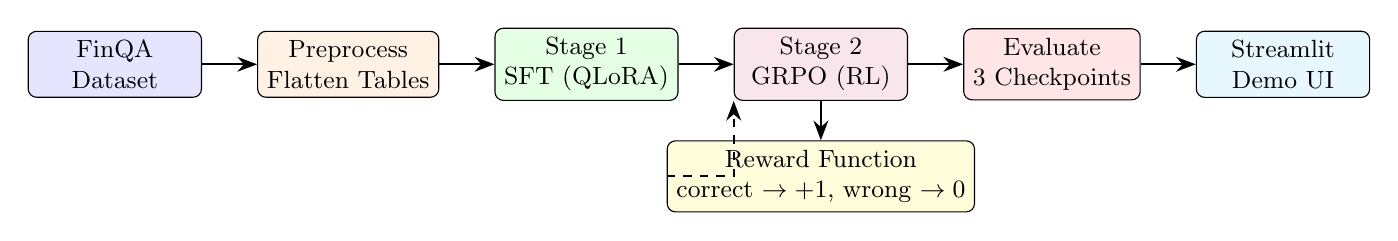
\begin{tikzpicture}[
    node distance=0.6cm and 0.7cm,
    box/.style={rectangle, draw, rounded corners=3pt, minimum width=2.2cm, minimum height=0.8cm, align=center, font=\small},
    arrow/.style={-{Stealth[length=2.5mm]}, thick},
]
    % Row 1: Data flow
    \node[box, fill=blue!10] (data) {FinQA\\Dataset};
    \node[box, fill=orange!10, right=of data] (prep) {Preprocess\\Flatten Tables};
    \node[box, fill=green!10, right=of prep] (sft) {Stage 1\\SFT (QLoRA)};
    \node[box, fill=purple!10, right=of sft] (grpo) {Stage 2\\GRPO (RL)};
    \node[box, fill=red!10, right=of grpo] (eval) {Evaluate\\3 Checkpoints};
    \node[box, fill=cyan!10, right=of eval] (ui) {Streamlit\\Demo UI};
    
    \draw[arrow] (data) -- (prep);
    \draw[arrow] (prep) -- (sft);
    \draw[arrow] (sft) -- (grpo);
    \draw[arrow] (grpo) -- (eval);
    \draw[arrow] (eval) -- (ui);
    
    % Reward loop
    \node[box, fill=yellow!15, below=0.5cm of grpo, minimum width=2.5cm] (reward) {Reward Function\\correct $\to +1$, wrong $\to 0$};
    \draw[arrow] (grpo.south) -- (reward.north);
    \draw[arrow, dashed] (reward.west) -| (grpo.south west);
    
\end{tikzpicture}
\end{center}

\subsection{Algorithms and Frameworks}

\textbf{Base Model:} Qwen2.5-1.5B-Instruct in 4-bit NF4 quantization (fits 8\,GB VRAM). Fallback: Phi-4-mini (3.8B) on Colab.

\textbf{Stage 1 (SFT):} QLoRA fine-tuning (rank 16, $\alpha{=}32$) using HuggingFace TRL's \texttt{SFTTrainer}. Teaches the model to parse financial tables and produce short answers.

\textbf{Stage 2 (GRPO):} Group Relative Policy Optimization via TRL's \texttt{GRPOTrainer} or Unsloth. For each question, 4 completions are sampled, scored by the deterministic reward function, and policy-updated using z-score normalized advantages. The prompt instructs step-by-step reasoning in \texttt{<think>} tags.

\textbf{Framework Stack:} PyTorch 2.x, HuggingFace Transformers, TRL, PEFT, bitsandbytes, Unsloth (optional), Streamlit.

\section{d. User Interface Plan}

\subsection{Input/Output Design}

\begin{tabularx}{\textwidth}{@{}lX@{}}
\toprule
\textbf{Component} & \textbf{Description} \\
\midrule
\textbf{User Input} & Paste or upload financial table/text + type a natural language question \\
\textbf{Model Output} & Extracted numerical answer, displayed prominently \\
\textbf{Reasoning Trace} & If the model produced \texttt{<think>} tags, the step-by-step reasoning is shown in an expandable info box \\
\textbf{Ground Truth Check} & Optional: user enters the correct answer, system shows ✓/✗ and the reward score \\
\textbf{Checkpoint Toggle} & Sidebar radio buttons to switch between Zero-Shot / SFT / GRPO and compare outputs live \\
\textbf{Results Dashboard} & Bottom section shows accuracy metrics and all 4 analysis figures from the evaluation \\
\bottomrule
\end{tabularx}

\subsection{Wireframe}

\begin{center}
\begin{tikzpicture}[
    frame/.style={rectangle, draw, minimum width=6cm, minimum height=3cm, align=center, font=\small},
    small/.style={rectangle, draw, minimum width=2.5cm, minimum height=0.6cm, align=center, font=\footnotesize},
]
    % Main layout
    \node[frame, minimum width=12cm, minimum height=5cm] (main) {};
    \node[anchor=north west, font=\small\bfseries] at ([shift={(0.2,-0.1)}]main.north west) {FinReason Demo};
    
    % Left panel
    \node[small, fill=gray!10, minimum width=5cm, minimum height=1cm] at (-2, 1.2) (input) {Financial Data (text area)};
    \node[small, fill=gray!10, minimum width=5cm] at (-2, 0.2) (question) {Question input};
    \node[small, fill=blue!15, minimum width=2cm] at (-2, -0.4) (btn) {Ask FinReason};
    
    % Right panel
    \node[small, fill=green!10, minimum width=4cm, minimum height=0.6cm] at (3.2, 1.2) (answer) {Answer: \textbf{306.2}};
    \node[small, fill=purple!8, minimum width=4cm, minimum height=1.2cm] at (3.2, 0.1) (think) {\texttt{<think>} reasoning};
    \node[small, fill=red!8, minimum width=4cm] at (3.2, -0.8) (check) {✓ Correct (R=1.2)};
    
    % Sidebar
    \node[small, fill=yellow!10, minimum width=2cm, minimum height=2.5cm, anchor=east] at ([shift={(-0.15,0)}]main.west) (sidebar) {Model\\Toggle:\\○ Zero-shot\\○ SFT\\● GRPO};

\end{tikzpicture}
\end{center}

\textbf{Technology:} Streamlit. Already implemented in \texttt{ui/app.py}. Runs with \texttt{streamlit run ui/app.py}.

\section{e. Innovation and Anticipated Challenges}

\textbf{What's new:} GRPO has been validated on clean math benchmarks (GSM8K, AIME). Applying it to real-world financial tables---with noisy formatting, unit ambiguity, and domain-specific computation---tests whether RLVR generalises beyond synthetic problems. Running it on a 1.5B model tests the lower bound of where RL-based reasoning works.

\textbf{C1. Reward sparsity.} If the 1.5B model rarely produces correct answers, GRPO gets zero gradient signal. \textit{Mitigation:} SFT warmup first; curriculum ordering (easy$\to$hard questions); increase group size from 4 to 8.

\textbf{C2. Fragile number parsing.} Financial outputs like ``\$1.45B'' or ``(3.5)'' must be parsed correctly or the reward function gives corrupted signal. \textit{Mitigation:} Exhaustive unit testing on 200+ edge cases before training.

\textbf{C3. TRL API instability.} The \texttt{GRPOTrainer} API has changed between TRL versions. \textit{Mitigation:} Pin TRL version in \texttt{requirements.txt}; maintain a manual GRPO fallback loop.

\section{f. Implementation Timeline}

\renewcommand{\arraystretch}{1.2}
\begin{tabularx}{\textwidth}{@{}p{2.5cm}p{4.5cm}X@{}}
\toprule
\textbf{Week} & \textbf{Focus} & \textbf{Expected Outcome} \\
\midrule
Apr 1--5 & Data loading, exploration, environment setup, reward function testing & Working \texttt{setup.ipynb} with verified data pipeline, all self-tests passing \\
Apr 5--12 & SFT training (Stage 1), zero-shot baseline, SFT evaluation & Checkpoints 1 and 2; measurable accuracy improvement over zero-shot \\
Apr 12--19 & GRPO training (Stage 2), reward tuning, hyperparameter search & Checkpoint 3; GRPO accuracy measured; training curves plotted \\
Apr 19--26 & Streamlit UI integration, ablation analysis, TAT-QA OOD test, figures & Interactive demo running; all 4 report figures generated \\
Apr 26--29 & Final report writing, code cleanup, presentation prep & Completed project, polished repo, presentation ready \\
\bottomrule
\end{tabularx}

\section{g. Responsible AI Reflection}

\textbf{Fairness:} FinQA is derived exclusively from S\&P 500 companies---large-cap US firms. The model may not generalise to financial statements from smaller companies, emerging markets, or non-English filings. Any deployment should be validated on the target population.

\textbf{Transparency:} The \texttt{<think>} reasoning traces provide a degree of interpretability: users can see \textit{why} the model produced a particular number, not just the number itself. The Streamlit UI exposes this reasoning directly.

\textbf{Environmental cost:} Total training compute is modest: ${\sim}$6--8 GPU-hours on a single consumer GPU, well below the threshold of frontier model training. The use of 4-bit quantization and QLoRA minimises energy consumption relative to full fine-tuning.

\textbf{Misuse risk:} A model that answers financial questions could produce incorrect outputs that are acted upon in real financial decisions. The system should be positioned as an \textit{assistant} tool, not an autonomous decision-maker, and all outputs should carry a disclaimer that they are AI-generated and require human verification.

\end{document}
